\documentclass[list,mac,answers]{BHCexam}
\pagestyle{fancy}
\fancyfoot[C]{\kaishu \small 第 \thepage 页 共 \pageref{lastpage} 页}
\fancyhead[L]{
\includegraphics[width=2cm]{qrcode.png}}
\begin{document}
\textbf{绝密\ding{72}启用前} 
\title{2020 年普通高等学校招生全国统一考试}
\subtitle{理科综合能力测试}
\maketitle

\textbf{注意事项:} 
\setlength\parindent{2em}

1. 答卷前,考生务必将自己的姓名、准考证号填写在答题卡上。

2. 回答选择题时,选出每小题答案后,用铅笔把答题卡上对应题目的答案标号涂黑,如需改动,用橡皮擦干净后,再选涂其它答案标号。回答非选择题时,将答案写在答题卡上,写在本试卷上无效。

3. 考试结束后,将本试卷和答题卡一并交回。

\begin{groups}

\group{选择题}{本题共 8 小题,每小题 6 分。共 48 分。在每小题给出的四个选项中,第 14\textasciitilde 18 题只有一项符合题目要求,第 19\textasciitilde21 题有多项符合题目要求。全部选对的得 6 分,选对但不全的得 3 分,有选错的得0分。}

\begin{questions}[30s]
\question[6]行驶中的汽车如果发生剧烈碰撞,车内的安全气囊会被弹出并瞬间充满气体.若碰撞后汽车的速度在很短时间内减小为零,关于安全气囊在此过程中的作用,下列说法正确的是\key{D}
\fourchoices{增加了司机单位面积的受力大小}{减少了碰撞前后司机动量的变化量}{将司机的动能全部转换成汽车的动能}{延长了司机的受力时间并增大了司机的受力面积}
\begin{solution}{4cm}

\end{solution}



\question[6]火星的质量约为地球质量的$1/10,$半径约为地球半径的$1/2,$则同一物体在火星表面与在地球表面受到的引力的比值约为\key{B}
\fourchoices{$0.2$}{$0.4$}{$2.0$}{$2.5$}
\begin{solution}{4cm}

\end{solution}



\question[6]如图,一同学表演荡秋千.已知秋千的两根绳长均为$10m,$该同学和秋千踏板的总质量约为$50kg.$绳的质量忽略不计,当该同学荡到秋千支架的正下方时,速度大小为$8m/s,$此时每根绳子平均承受的拉力约为\key{B}
\begin{center}
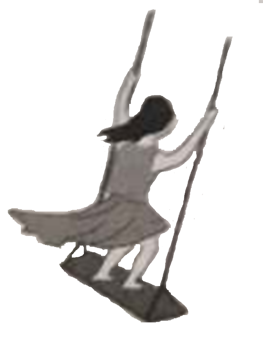
\includegraphics[]{img/image1.png}
\end{center}

\fourchoices{$200N$}{$400N$}{$600N$}{$800N$}
\begin{solution}{4cm}

\end{solution}


\newpage
\question[6]图(a)所示的电路中,K与L间接一智能电源,用以控制电容器C两端的电压$U_C.$如果$U_C$随时间t的变化如图(b)所示,则下列描述电阻R两端电压$U_R$随时间t变化的图像中,正确的是\key{A}
\begin{center}
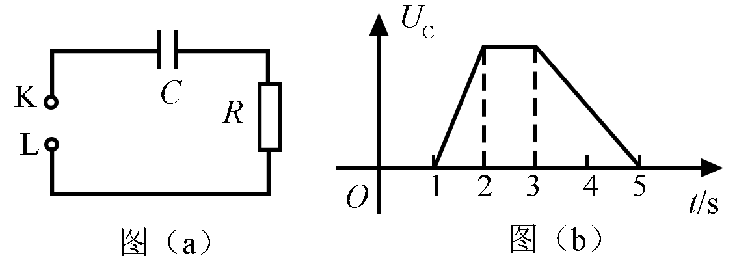
\includegraphics[width=8cm]{img/image2.png}
\end{center}
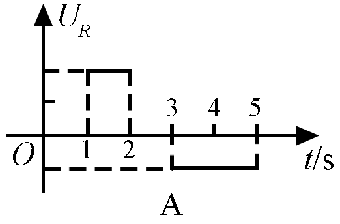
\includegraphics[width=3.5cm]{img/image3.png}
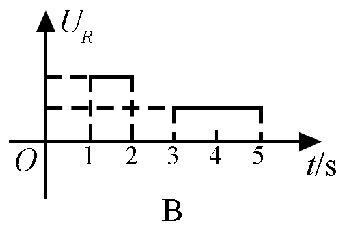
\includegraphics[width=3.5cm]{img/image4.png}
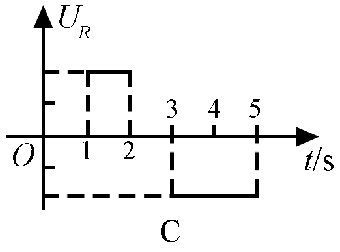
\includegraphics[width=3.5cm]{img/image5.png}
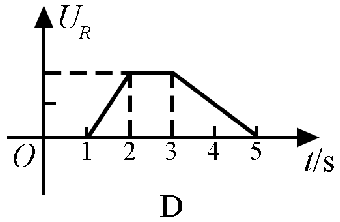
\includegraphics[width=3.5cm]{img/image6.png}

\begin{solution}{4cm}

\end{solution}



\question[6]一匀强磁场的磁感应强度大小为B,方向垂直于纸面向外,其边界如图中虚线所示$,ab$为半圆$,ac、bd$与直径ab共线$,ac$间的距离等于半圆的半径.一束质量为m、电荷量为$q(q>0)$的粒子,在纸面内从c点垂直于ac射入磁场,这些粒子具有各种速率.不计粒子之间的相互作用.在磁场中运动时间最长的粒子,其运动时间为\key{C}
\begin{center}
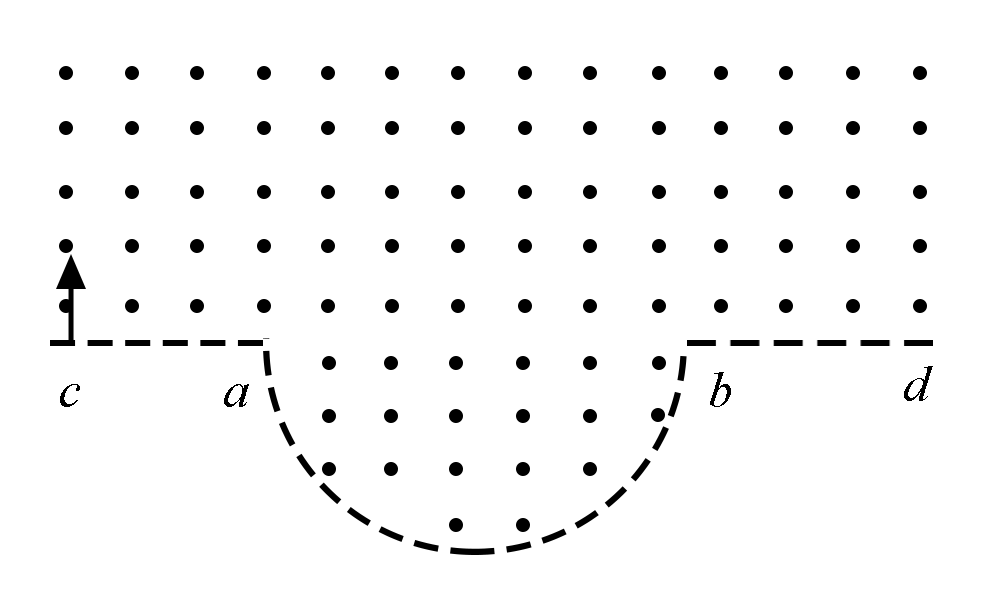
\includegraphics[]{img/image7.png}
\end{center}

\fourchoices{$\frac{7\pi m}{6qB}$}{$\frac{5\pi m}{4qB}$}{$\frac{4\pi m}{3qB}$}{$\frac{3\pi m}{2qB}$}
\begin{solution}{4cm}

\end{solution}



\question[6]下列核反应方程中$,X_1,X_2,X_3,X_4$代表α粒子的有\key{BD}
\fourchoices{$_1^2H+_1^2H→_0^10^n+X_1$}{$^{2}_{1}H+_{1}^{3}H\rightarrow_{0}^{1}n+X_{2}$}{$_{92}^{235}U+_{0}^{1}n\rightarrow_{56}^{144}Ba+\frac{89}{36}Kr+3X_{3}$}{$_{0}^{1}n+\frac{6}{3}Li\rightarrow_{1}^{3}H+X_{4}$}
\begin{solution}{4cm}

\end{solution}


\newpage
\question[6]一物块在高$3.0m$、长$5.0m$的斜面顶端从静止开始沿斜面下滑,其重力势能和动能随下滑距离s的变化如图中直线\uppercase\expandafter{\romannumeral1}、\uppercase\expandafter{\romannumeral2 }所示,重力加速度取$10m/s^2.$则\key{AB}
\begin{center}
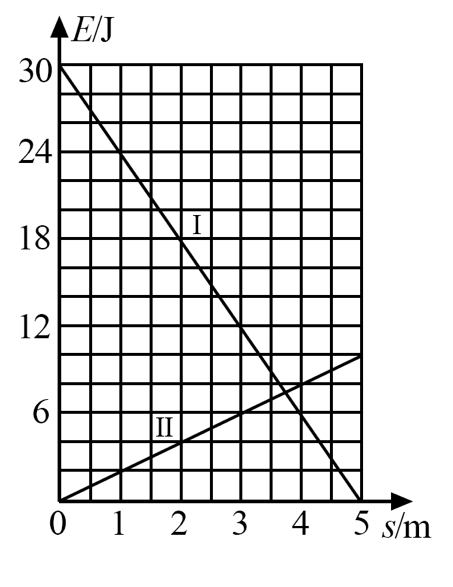
\includegraphics[]{img/image8.png}
\end{center}

\fourchoices{物块下滑过程中机械能不守恒}{物块与斜面间的动摩擦因数为$0.5$}{物块下滑时加速度的大小为$6.0m/s^2$}{当物块下滑$2.0m$时机械能损失了$12J$}
\begin{solution}{4cm}

\end{solution}



\question[6]如图,U形光滑金属框$abcd$置于水平绝缘平台上$,ab$和dc边平行,和bc边垂直$.ab$、$dc$足够长,整个金属框电阻可忽略.一根具有一定电阻的导体棒MN置于金属框上,用水平恒力F向右拉动金属框,运动过程中,装置始终处于竖直向下的匀强磁场中$,MN$与金属框保持良好接触,且与bc边保持平行.经过一段时间后\key{BC}
\begin{center}
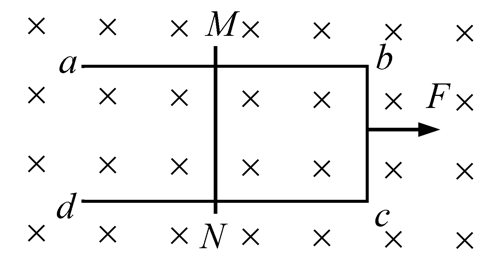
\includegraphics[]{img/image9.png}
\end{center}

\fourchoices{属框的速度大小趋于恒定值}{属框的加速度大小趋于恒定值}{体棒所受安培力的大小趋于恒定值}{体棒到金属框bc边的距离趋于恒定值}
\begin{solution}{4cm}

\end{solution}
\newpage



\end{questions}

\group{非选择题}{共 174 分,第 22\textasciitilde 32 题为必考题,每个试题考生都必须作答。第 33\textasciitilde38 题为选考题,考生根 据要求作答。}

\begin{questions}[p]
\question[6] $13.(6$分)如图所示装置可以用来研究小车的匀变速直线运动.带有定滑轮的长木板放置在桌面上,重物通过跨过定滑轮的细线拉着小车向左加速运动,定滑轮与小车间的细线与长木板平行,打点计时器打下的纸带记录下小车的运动信息.
(1)下面说法正确的是$.A.$长木板必须水平放置B.小车的质量必须远大于重物的质量纸带$C.$需要平衡小车与长木板间的摩擦力D.应该先接通打点计时器的电源,然后再释放小车
(2)实验时将打点计时器接到频率为$50Hz$的交流电源上,选取一条点迹清晰的纸带,在纸带上每隔四个点取一个计数点,测出相邻计数点间的距离如图所示,其中$x_1=5.09cm,x_2=7.10cm,x_3=9.10cm,x_4=11.10cm,x_5=13.09cm,x_s=15.10cm.$则打第4个计数点时小车的速度$v_4=_m/s,$小车的加速度$a=_m/s^2($结果均保留两位有效数字).
\begin{center}
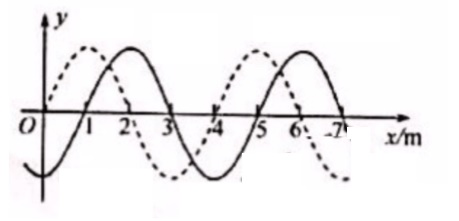
\includegraphics[]{img/image13.jpeg}
\end{center}

\question[6] $14.(9$分)某同学用如图所示装置做"探究加速度与合力关系"的实验.测得小车(带遮光片)的质量为M,当地的重力加速度为$g.\frac{2}{1}cm⊥$砂桶1020
(1)实验前,用游标卡尺测出遮光片的宽度,示数如图所示,则遮光片的宽度为d=cm.
(2)为了使细线的拉力近似等于砂和砂桶的总重力,必须$_—°A.$将长木板的右端适当垫高,以平衡摩擦力B.砂和砂桶的总质量远小于小车的质量C.使连接小车的细线与长木板平行D.减小遮光片的宽度
(3)调节好装置,将小车由静止释放,与光电门连接的计时器显示小车通过光电门时遮光片的遮光时间t,要测量小车运动的加速度,还需要测量$($填写需要测量的物理量名称),若该物理量用x表示,则小车运动的加速度大小为$($用测得的物理量符号表示).
(4)保持小车每次释放的位置不变,光电门的位置不变,改变砂和砂桶的总质量,重复实验,测得多组小百投翻联显$2020$届$TOP300$七月尖子生联考物理第3页"共6页车通过光电门的遮光时间t及砂和砂桶的总质量m.为了使图象能直观地反映物理量之间的关系.应该作出($(-t^{\prime\prime},m-\frac{1}{t}m-t^{2},\cdots m-\frac{1}{t^{2}}y$图象.当图象为过原点的一条倾斜的直线,表明质量一定时加速度与合力成正比.
\question[6] $15.(8$分)某物体沿着一条直线做匀减速运动.途经$A.B.C$三点,最终停止在D点$.A、B$之间的距离为$s B.C$之间的距离为 号$\frac{2}{3}s_{0}$物体通过AB与BC两段距离所用时间都为t…求:
(1)物体经过A点时的速度,Aiⅳc―b
(2)物体经过CD段的平均速度.百以固获生$2020$届$TOP00$七月尖子生联考物理第4页共6页
\question[6] $16.(11$分)如图所示.质量为$m=6kg,$足够长的长木板放在水平面上,其上表面水平.质量为$m_1=3kg$的物块A放在长木板上距板右端$L,=3m$处,质量为$m=3kα$的物块B放在长木板上左端.地面上离长的$=,_=$原图的二一
下下面平下列的 新出Ⅱ两气出A是得重是重的的=体图关色是不W的数用图新此正要用假的物对脱离个假已知四物块与长木板间的动摩擦因数均为$\mu_1=0.5,$长木板与地面间的动摩擦因数为
$\mu_2=0.1,$重力加速度$g=10m/s^∘,$最大静摩擦力等于滑动摩擦力,不计物块大小,求拉力F的大小$. _v─r. $
\question[6] $17.(13$分)质量为$1kg$的小型无人机下面悬挂着一个质量为$0.5kg$的小物块,正以$2m/s$的速度匀速下降,某时刻悬绳断裂小物块竖直下落,小物块经过2s落地,已知无人机运动中受到的空气阻力大小始终为其自身重力的$0.1$倍,无人机的升力始终恒定,不计小物块受到的空气阻力,重力加速度为$10m/s,$求出小物地刚要落地时$."'0¥10$的.O生人能到地面的高度.
(2)无人机离3百以固获生$2020$届$TOP00$七月尖子生联考物理第5页共6页
\question[6] $18.15$分)如图所示,倾角为$37^°$的斜面体固定在水平面上,斜面上$A、B$两个位置之间的距离为$2m.$第一次用沿斜面向上,大小为$F=6N$的力把质量为$0.5kg$的物体由静止从A处拉到B处.所用时间为$1s,$第段时间二场上$A+,$物是实验到B
从$_"$
时上 重石眼至不分物体运动到B处时速度刚好减为零.已知$sin37=0.6,cos37=0.8,$不计物体大小,重力m区段器二0"常有的因数,
(1)物体与斜面间的动摩擦因数.
(2)物体第二次从A运动到B的过程·水平力F的作用时间.(结果可保留根式)百以固获生$2020$届$TOP00$七月尖子生联考物理第5页共6页$18.15$分)如图所示,倾角为$37^°$的斜面体固定在水平面上,斜面上$A、B$两个位置之间的距离为$2m.$第一次用沿斜面向上,大小为$F=6N$的力把质量为$0.5kg$的物体由静止从A处拉到B处.所用时间为$1s,$第段时间二场上$A+,$物是实验到B从$_"$时上 重石眼至不分物体运动到B处时速度刚好减为零.已知$sin37=0.6,cos37=0.8,$不计物体大小,重力m区段器二0"常有的因数,
(1)物体与斜面间的动摩擦因数.
(2)物体第二次从A运动到B的过程·水平力F的作用时间.(结果可保留根式)
\begin{center}
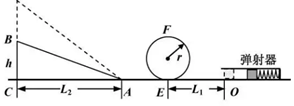
\includegraphics[]{img/image18.jpeg}
\end{center}


\end{questions}



\end{groups}
\label{lastpage}
\end{document}
